\documentclass[10pt,letterpaper]{article}
\usepackage{amsmath}
\usepackage{amsfonts}
\usepackage{amssymb}
\usepackage[utf8]{inputenc}
\usepackage{makeidx}
\usepackage{graphicx}
\usepackage{lmodern}
\usepackage[left=2cm,right=2cm,top=2cm,bottom=2cm]{geometry}
%Used for color for programming language
\usepackage{listings}
\usepackage{color}
\usepackage{graphicx}
\usepackage{subcaption}
\usepackage{float}

\newcommand{\hmwkTitle}{Assignment\ \#5} % Assignment title
\newcommand{\hmwkDueDate}{11:59pm March 7,\ 2018} % Due date
\newcommand{\hmwkClass}{CS 535} % Course/class
\newcommand{\hmwkClassTime}{16:20} % Class/lecture time
\newcommand{\hmwkClassInstructor}{Alexander C. Nwala} % Teacher/lecturer
\newcommand{\hmwkAuthorName}{David Sinclair} % Your name

%----------------------------------------------------------------------------------------
%	TITLE PAGE
%----------------------------------------------------------------------------------------

\title{
\vspace{2in}
\textmd{\textbf{\hmwkClass:\ \hmwkTitle}}\\
\normalsize\vspace{0.1in}\small{Due\ on\ \hmwkDueDate}\\
\vspace{0.1in}\large{\textit{\hmwkClassInstructor\ \hmwkClassTime}}
\vspace{3in}
}
\author{\textbf{\hmwkAuthorName}}


\begin{document}

\maketitle
%----------------------------------------------------------------------------------------
%	TABLE OF CONTENTS
%----------------------------------------------------------------------------------------

%\setcounter{tocdepth}{1} % Uncomment this line if you don't want subsections listed in the ToC

\pagebreak
\tableofcontents
\pagebreak 

%----------------------------------------------------------------------------------------
%	Create colors for scripting 
%----------------------------------------------------------------------------------------


\definecolor{dkgreen}{rgb}{0,0.6,0}
\definecolor{gray}{rgb}{0.5,0.5,0.5}
\definecolor{mauve}{rgb}{0.58,0,0.82}

\lstset{frame=tb,
  language=Python,
  aboveskip=3mm,
  belowskip=3mm,
  showstringspaces=false,
  columns=flexible,
  basicstyle={\small\ttfamily},
  numbers=none,
  numberstyle=\tiny\color{gray},
  keywordstyle=\color{blue},
  commentstyle=\color{dkgreen},
  stringstyle=\color{mauve},
  breaklines=true,
  breakatwhitespace=true,
  tabsize=3
}
%----------------------------------------------------------------------------------------
%	Problem 1 %----------------------------------------------------------------------------------------

\section{Problem 1}
\subsection{Question 1}
1.  We know the result of the Karate Club (Zachary, 1977) split.
Prove or disprove that the result of split could have been predicted
by the weighted graph of social interactions.  How well does the
mathematical model represent reality?\\
\\
Generously document your answer with all supporting equations, code,
graphs, arguments, etc.\\
\\
Clues: \\
1. Draw original Karate club graph (two connected components) after split (Week 6 lecture, slide 98).\\
2. Run multiple iterations of graph partitioning algorithm (e.g., Girvan-Newman Algorithm) on experimental Karate club graph until the graph splits into two connected components.\\
3. Compare the connected components of the experimental graph (in 2.) with the original connected components of the split Karate club graph (in 1.). Are they similar?\\
\\
Useful sources include:\\
\\
* Original paper\\
\\
http://aris.ss.uci.edu/~lin/76.pdf\\
\\
* Week 6 Slides:\\
\\
https://docs.google.com/presentation/d/1ihf6N8bHgzM5VLAyHkmF\_i5JGUBVpCSdsvYpk8XgHwo/edit?usp=sharing
\\
* Slides\\
\\
http://www-personal.umich.edu/~ladamic/courses/networks/si614w06/ppt/lecture18.ppt\\
\\
http://clair.si.umich.edu/si767/papers/Week03/Community/CommunityDetection.pptx\\
\\
* Code and data\\
\\
https://networkx.github.io/documentation/networkx\-1.10/reference/generated/networkx.generators.social.karate\_club\_graph.html\\
\\
https://networkx.github.io/documentation/networkx\-1.9/examples/graph/karate\_club.html\\
\\
http://nbviewer.ipython.org/url/courses.cit.cornell.edu/info6010/resources/11notes.ipynb\\
\\
http://stackoverflow.com/questions/9471906/what\-are\-the\-differences\-between\-community\-detection\-algorithms\-in\-igraph/9478989\#9478989\\
\\
http://stackoverflow.com/questions/5822265/are\-there\-implementations\-of\-algorithms\-for\-community\-detection\-in\-graphs\\
\\
http://konect.uni\-koblenz.de/networks/ucidata\-zachary\\
\\
http://vlado.fmf.uni\-lj.si/pub/networks/data/ucinet/ucidata.htm\#zachary\\
\\
https://snap.stanford.edu/snappy/doc/reference/CommunityGirvanNewman.html\\
\\
http://igraph.org/python/doc/igraph\-pysrc.html\#Graph.community\_edge\_betweenness\\
\\
\pagebreak 
\subsection{Answer 1}

For this question I used the following program that I captured from two major sources.\\ 
\bibliography{assignment5}
@online{YouTube,
author = {IIT ROPAR},
title = {Lecture 36 Community Detection Using Girvan Newman Algorithm},
year = {Oct 8, 2017},
url = {https://www.youtube.com/watch?v=c27VEbGdgCg},
}
\\
@online{PythonCode,
author = {millionsmile/gist:3676569},
title = {Karate club community detection by Girvan-Newman algorithm: gistfile1.py },
year = {2012},
url = {https://gist.github.com/millionsmile/3676569},
}
\\
\\
After that I created the following code.  I wanted to first create the original graph.\\
\\
\begin{lstlisting}
G = nx.karate_club_graph()
count = 0
pos = nx.spring_layout(G)
output = "karate%(id)02d.png" % {"id": count}
print('The file # is ', count,file=open('edgeremove.txt','a'))
pl.figure()
nx.draw_networkx(G, pos)
\end{lstlisting}

This created figure \ref{fig:kart0} which shows the original club.\\
\\
\begin{figure}[h!]
  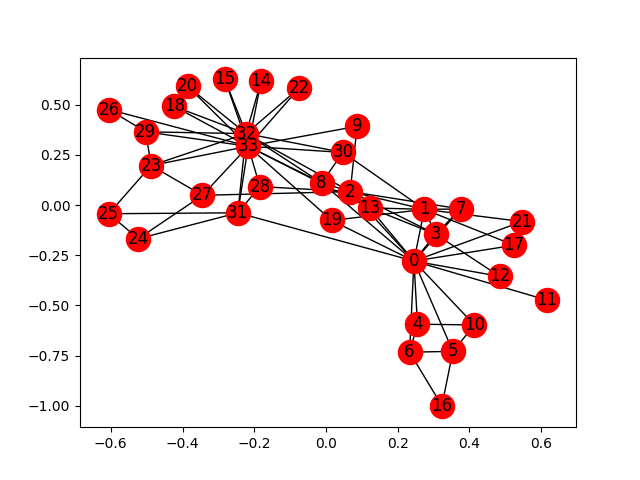
\includegraphics[width=\linewidth]{karate00.png}
  \caption{figure 0 Original Club}
  \label{fig:kart0}
\end{figure}
 
Know that I now I had my data correct.  I began using the Girvan-Newman algorithm to remove the highest edge of betweenness.  This is the code from the program that determined the highest edge of betweenness.\\
\\

\begin{lstlisting}
def edge_to_remove(G):
        dict1 = nx.edge_betweenness_centrality(G)
        list_of_tuples = dict1.items()
        list_of_tuples=sorted(list_of_tuples, key=lambda x:x[1], reverse=True)
        for x in list_of_tuples:
                return x[0]
\end{lstlisting}

Of note after getting the edge of betweenness values, it is important to sort the data from highest to lowest.  If that is not done then the data will not randomly select what to remove based on the values inserted from the beginning to the end not  taking into account weight or degree.\\
\\
Then comes the data of what points to remove and what the graph will look like.\\
\\
The rest of the program did this.\\
\\
\begin{lstlisting}
def girvan(G):
        c = nx.connected_component_subgraphs(G)
        l = len(list(c))
        pos = nx.spring_layout(G)
        count = 1
        print(count," The number connected compents are ",l)
        output = "karate%(id)02d.png" % {"id": count}
        print('The file # is ', count,' Edge that was removed: ',edge_to_remove(G), file=open('edgeremove.txt','a'))
        pl.figure()
        nx.draw_networkx(G, pos)
        pl.savefig(output)
        pl.close()
        while(l == 1):
                G.remove_edge(*edge_to_remove(G)) #((a,b)) --> (a,b)
                c = nx.connected_component_subgraphs(G)
                l = len(list(c))
                pos=nx.spring_layout(G)
                count +=1
                print(count, " The number connected compents are ",l)
                print('The file # is ', count,' Edge that was removed: ', edge_to_remove(G),file=open('edgeremove.txt','a'))
                output = "karate%(id)02d.png" % {"id": count}
                pl.figure()
                nx.draw_networkx(G, pos)
                pl.savefig(output)
                pl.close()

        return c
\end{lstlisting}

This created figure \ref{fig:kart1} which shows the progression by using the Girvan-Newman algorithm.\\
\\
\begin{figure}[H]
  \centering
  \begin{subfigure}[b]{0.4\linewidth}
     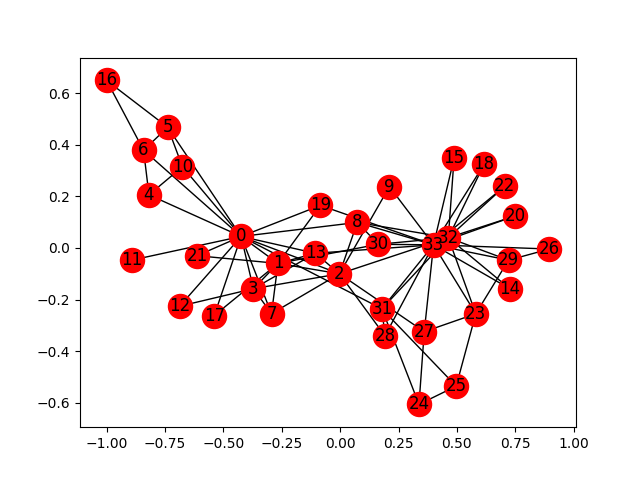
\includegraphics[width=\linewidth]{karate01.png}
     \caption{fig 1 had edge (0, 31) removed}
  \end{subfigure}
  \begin{subfigure}[b]{0.4\linewidth}
     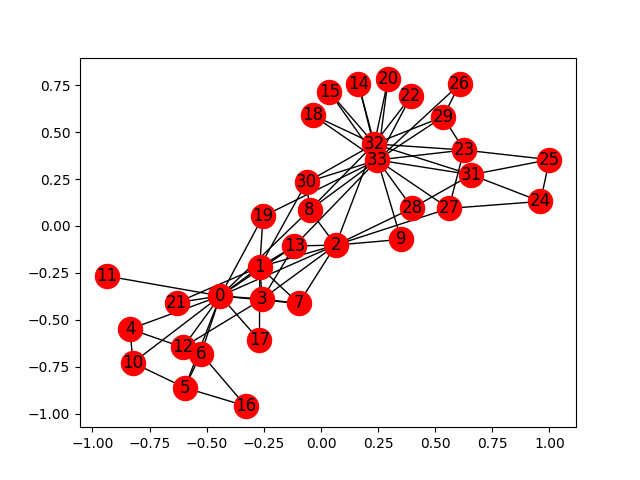
\includegraphics[width=\linewidth]{karate02.png} 
     \caption{fig 2 had edge (0, 2) removed}
  \end{subfigure}
  \begin{subfigure}[b]{0.4\linewidth}
     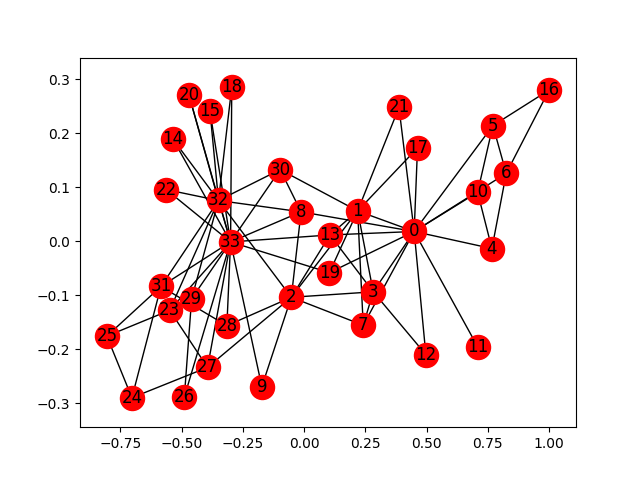
\includegraphics[width=\linewidth]{karate03.png} 
     \caption{fig 3 had edge (0, 8) removed}
  \end{subfigure}
   \begin{subfigure}[b]{0.4\linewidth}
     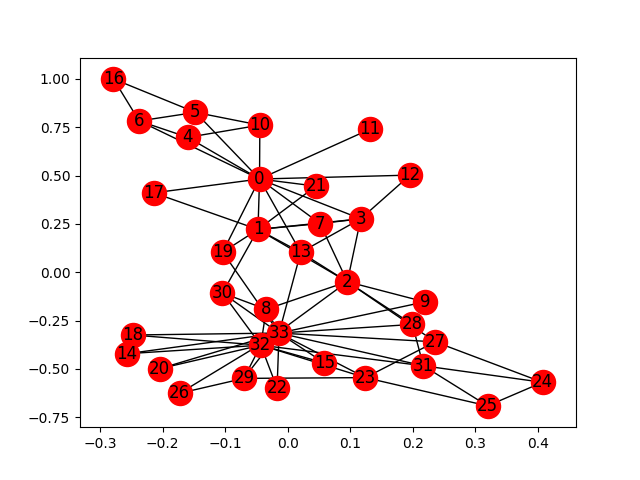
\includegraphics[width=\linewidth]{karate04.png} 
     \caption{fig 4 had edge (13, 33) removed}
  \end{subfigure}
   \begin{subfigure}[b]{0.4\linewidth}
     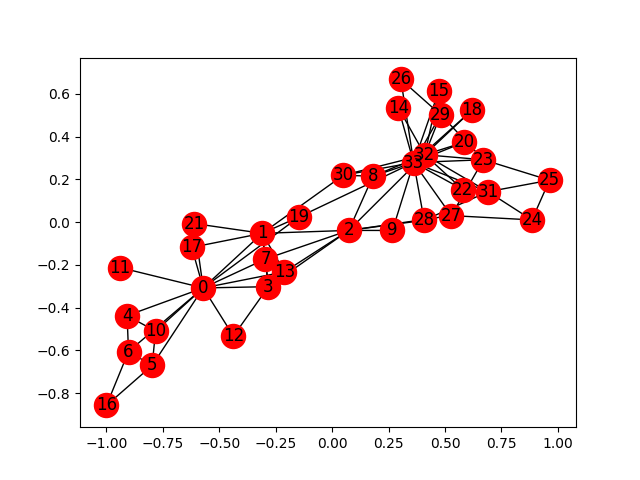
\includegraphics[width=\linewidth]{karate05.png} 
     \caption{fig 5 had edge (19, 33) removed}
  \end{subfigure}
   \begin{subfigure}[b]{0.4\linewidth}
     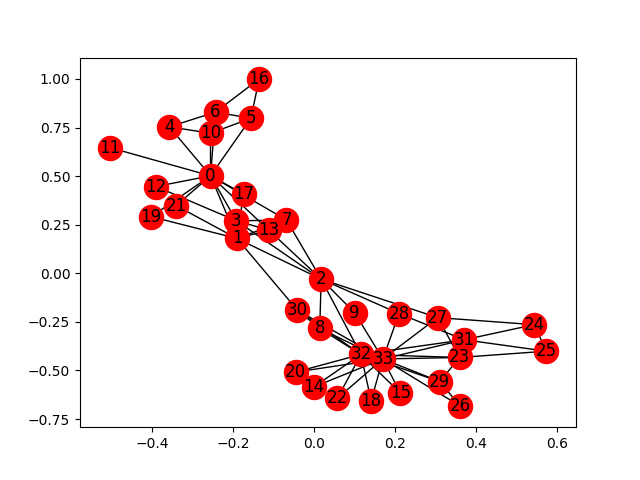
\includegraphics[width=\linewidth]{karate06.png} 
     \caption{fig 6 had edge (2, 32) removed}
  \end{subfigure}

  \caption{The karate club from 1977 moving to split.}
  \label{fig:kart1}
\end{figure}

Figures \ref{fig:kart2} continued up to 12 files.\\
\\
\begin{figure}[H]
  \centering
   \begin{subfigure}[b]{0.4\linewidth}
     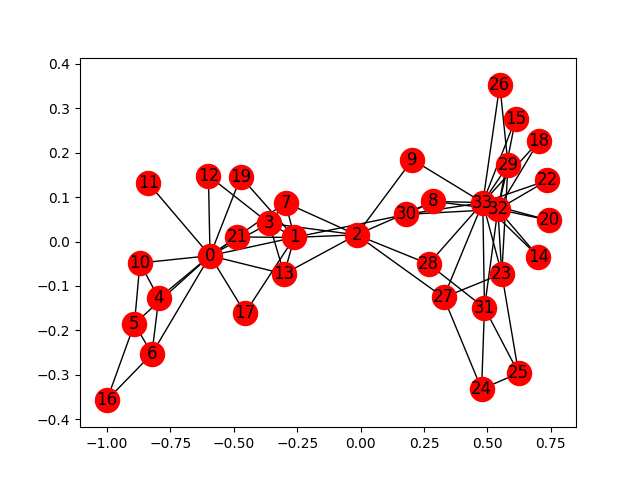
\includegraphics[width=\linewidth]{karate07.png} 
     \caption{fig 7 had edge (1, 30) removed}
  \end{subfigure}
   \begin{subfigure}[b]{0.4\linewidth}
     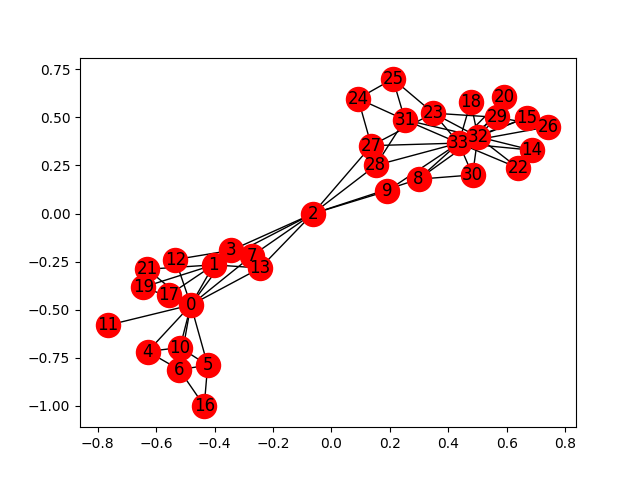
\includegraphics[width=\linewidth]{karate08.png} 
     \caption{fig 8 had edge (1, 2) removed}
  \end{subfigure}
   \begin{subfigure}[b]{0.4\linewidth}
     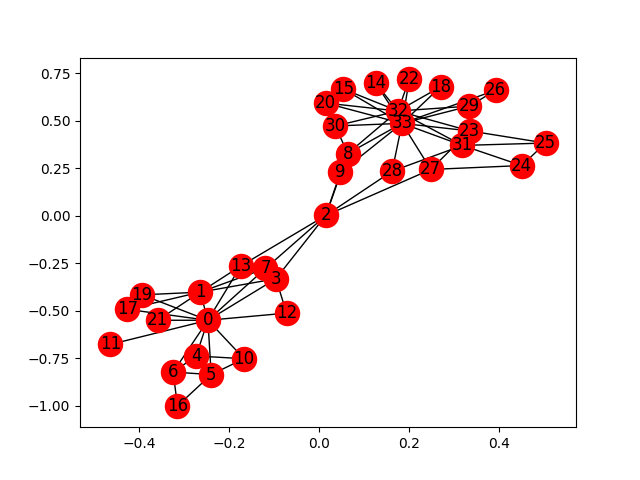
\includegraphics[width=\linewidth]{karate09.png} 
     \caption{fig 9 had edge (2, 3) removed}
  \end{subfigure}
   \begin{subfigure}[b]{0.4\linewidth}
     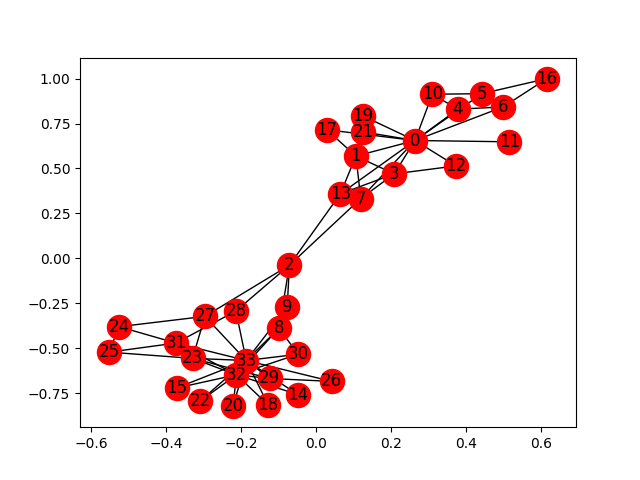
\includegraphics[width=\linewidth]{karate10.png} 
     \caption{fig 10 had edge (2, 13) removed}
  \end{subfigure}
   \begin{subfigure}[b]{0.4\linewidth}
     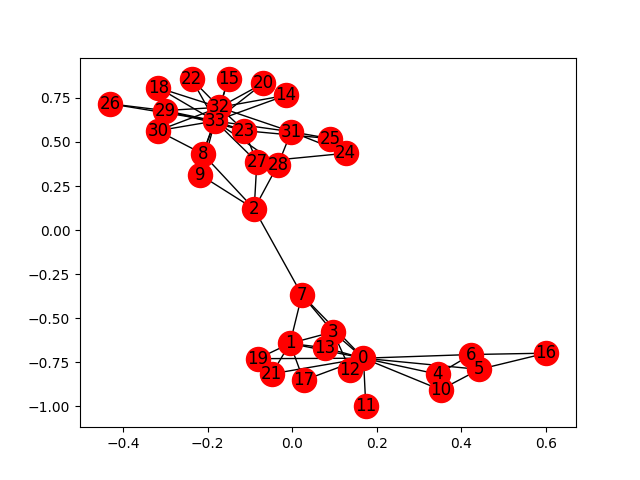
\includegraphics[width=\linewidth]{karate11.png} 
     \caption{fig 11 had edge (2, 7) removed}
  \end{subfigure}
   \begin{subfigure}[b]{0.4\linewidth}
     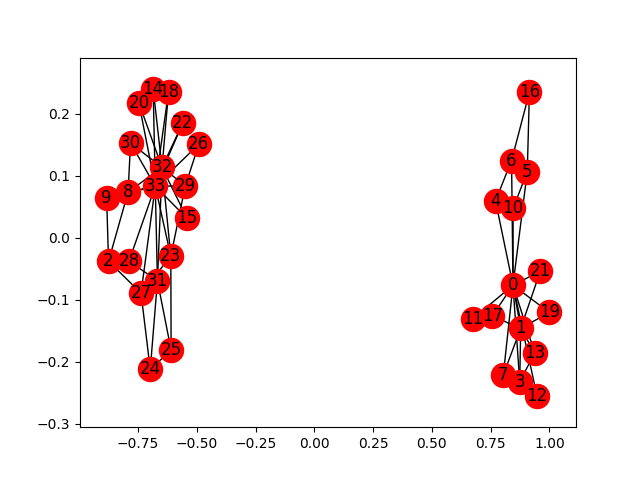
\includegraphics[width=\linewidth]{karate12.png} 
     \caption{fig 12 had edge (9, 33) removed}
  \end{subfigure}
  \caption{The karate club from 1977 moving to split (cont).}
  \label{fig:kart2}
\end{figure}
 
The above data will be called Edge Betweenness when I start comparing between the items I did and what was presented in class.\\
\\
This is all the information that I collected.  Now I will show you all the information from the power point slides that were presented in class.   This is listed in figures \/ slides \ref{fig:slid1}\\
\\
\begin{figure}[H]
  \centering
  \begin{subfigure}[b]{0.4\linewidth}
     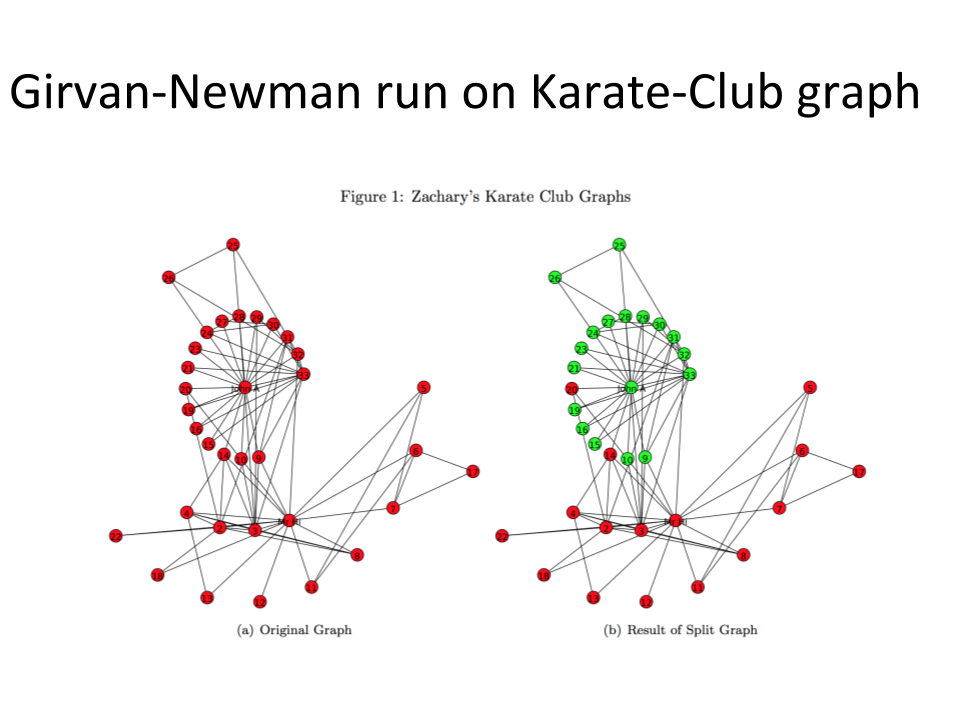
\includegraphics[width=\linewidth]{slide98.png}
     \caption{slide 1 Original information slide 98}
  \end{subfigure}
  \begin{subfigure}[b]{0.4\linewidth}
     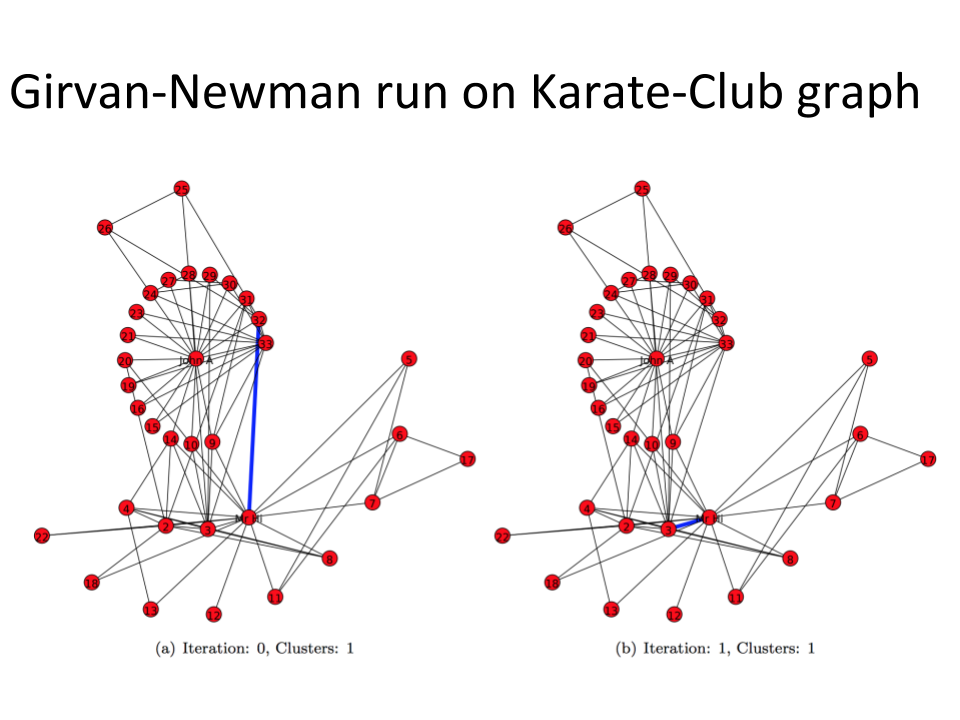
\includegraphics[width=\linewidth]{slide99.png} 
     \caption{slide 2 Original information slide 99}
  \end{subfigure}
  \begin{subfigure}[b]{0.4\linewidth}
     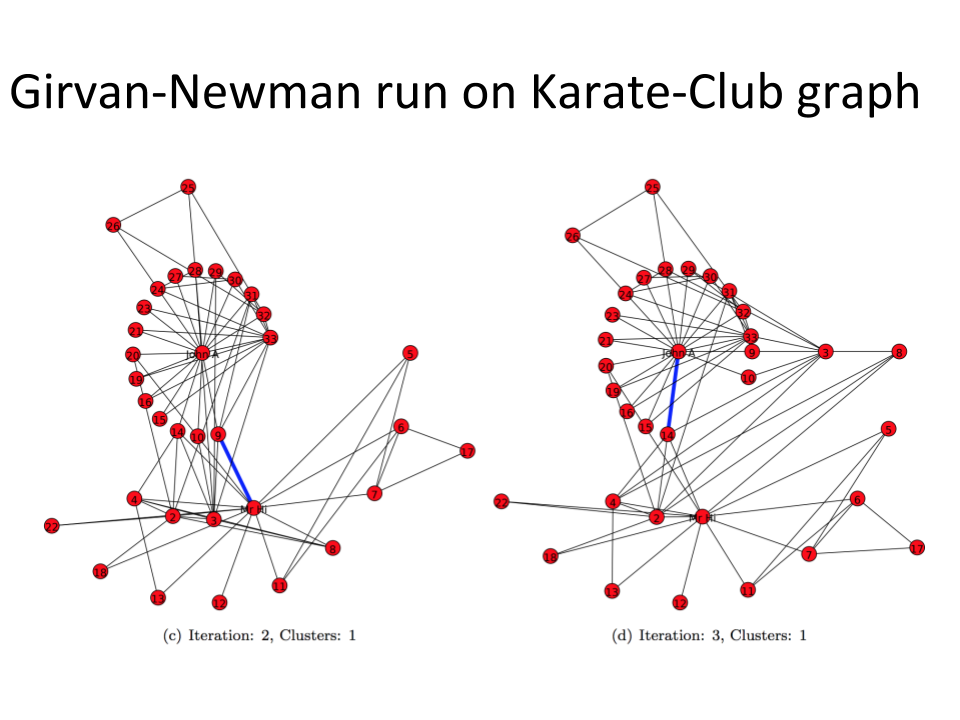
\includegraphics[width=\linewidth]{slide100.png} 
     \caption{slide 3 Original information slide 100}
  \end{subfigure}
  \begin{subfigure}[b]{0.4\linewidth}
     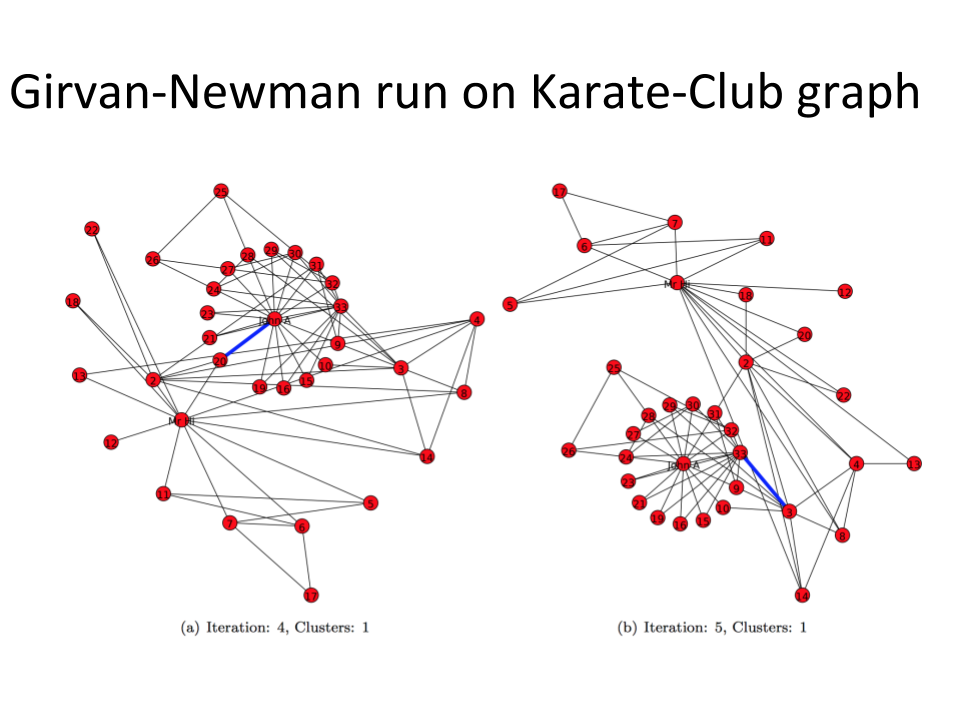
\includegraphics[width=\linewidth]{slide101.png} 
     \caption{slide 4 Original information slide 101}
  \end{subfigure}
  \begin{subfigure}[b]{0.4\linewidth}
     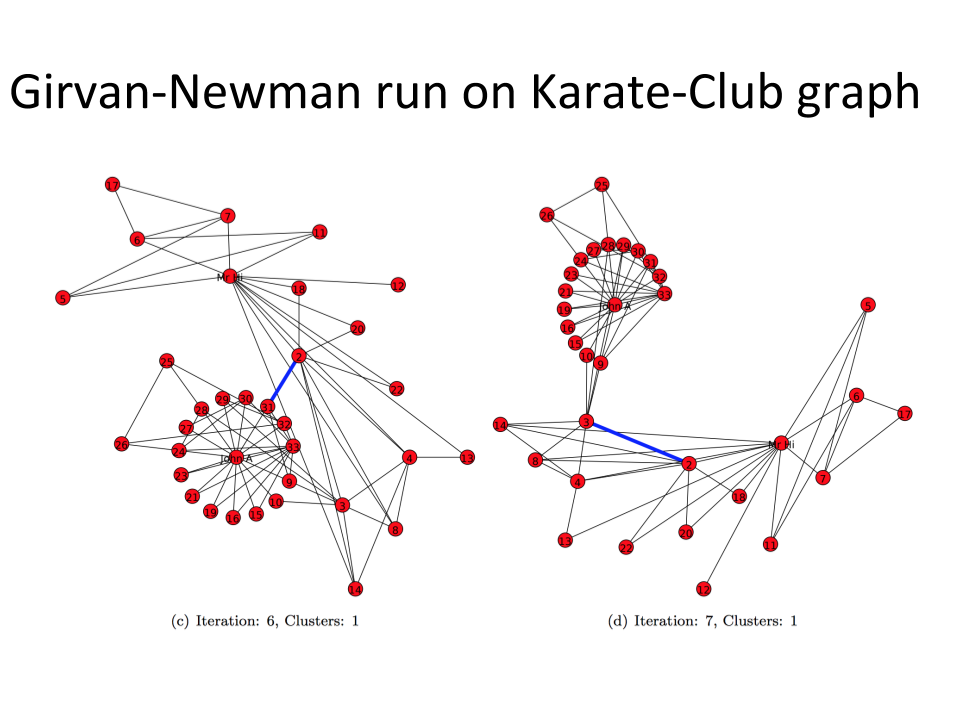
\includegraphics[width=\linewidth]{slide102.png} 
     \caption{slide 5 Original information slide 102}
  \end{subfigure}  
  \begin{subfigure}[b]{0.4\linewidth}
     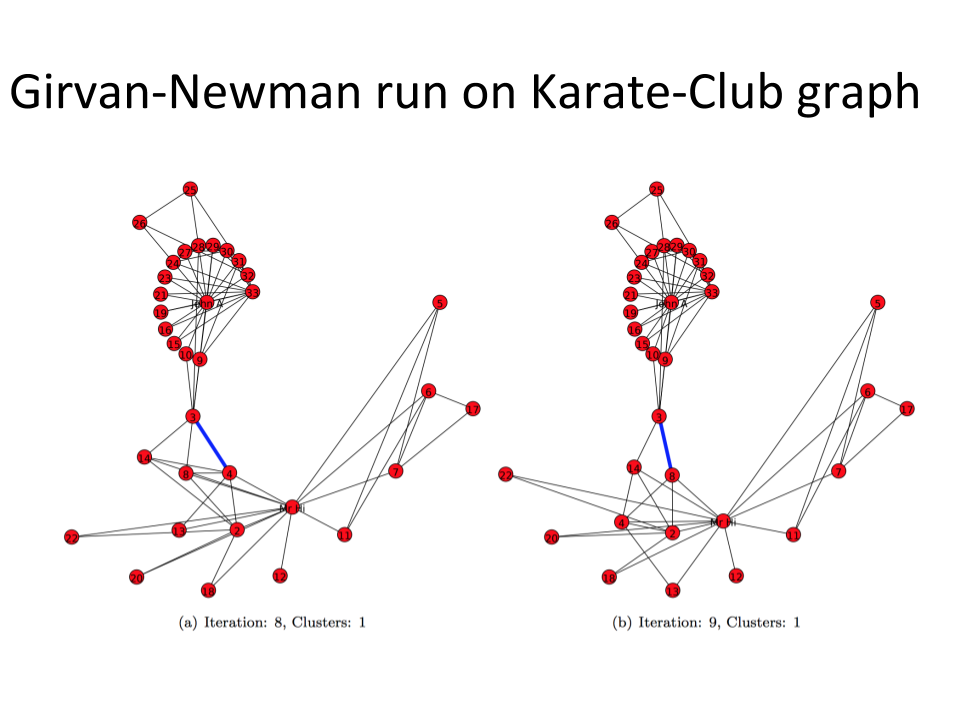
\includegraphics[width=\linewidth]{slide103.png} 
     \caption{slide 6 Original information slide 103}
  \end{subfigure}   
  \begin{subfigure}[b]{0.4\linewidth}
     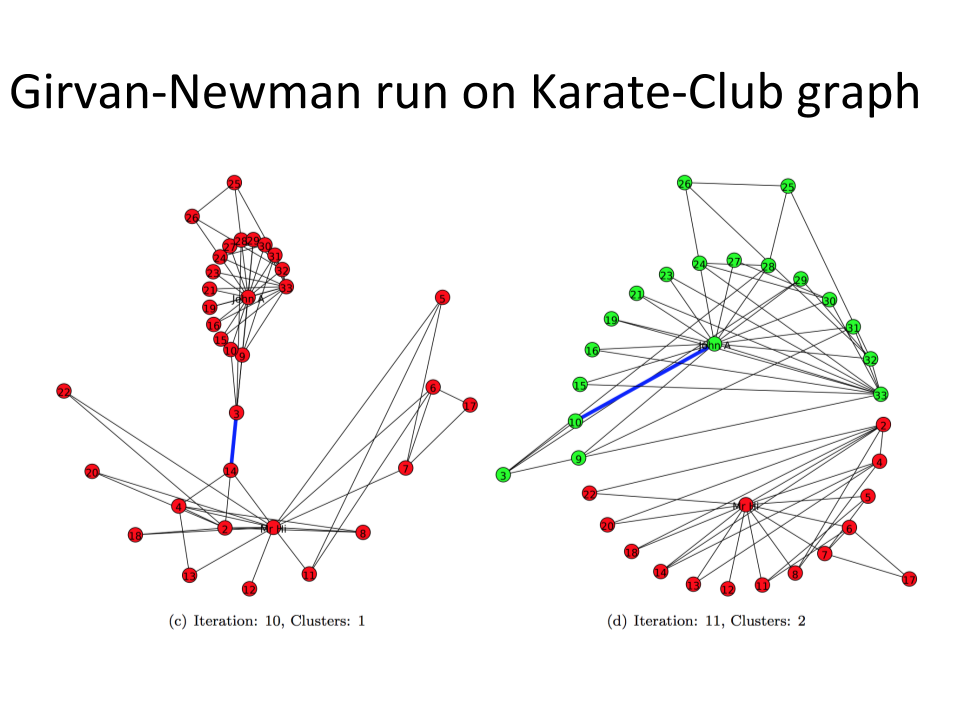
\includegraphics[width=\linewidth]{slide104.png} 
     \caption{slide 7 Original information slide 104}
  \end{subfigure}   
  \caption{The karate club from 1977 class lecture information.}
  \label{fig:slid1}
\end{figure}

Comparing the first graphs they do not look quite the same but the connections are the same.  This can be seen in figure \ref{fig:comp1}\\
\\
\begin{figure}[H]
  \centering
  \begin{subfigure}[b]{0.4\linewidth}
     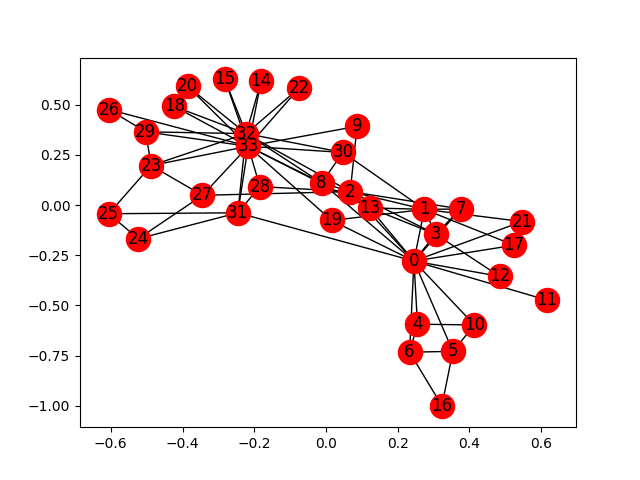
\includegraphics[width=\linewidth]{karate00.png}
     \caption{Edge Betweenness original data}
  \end{subfigure}
  \begin{subfigure}[b]{0.4\linewidth}
     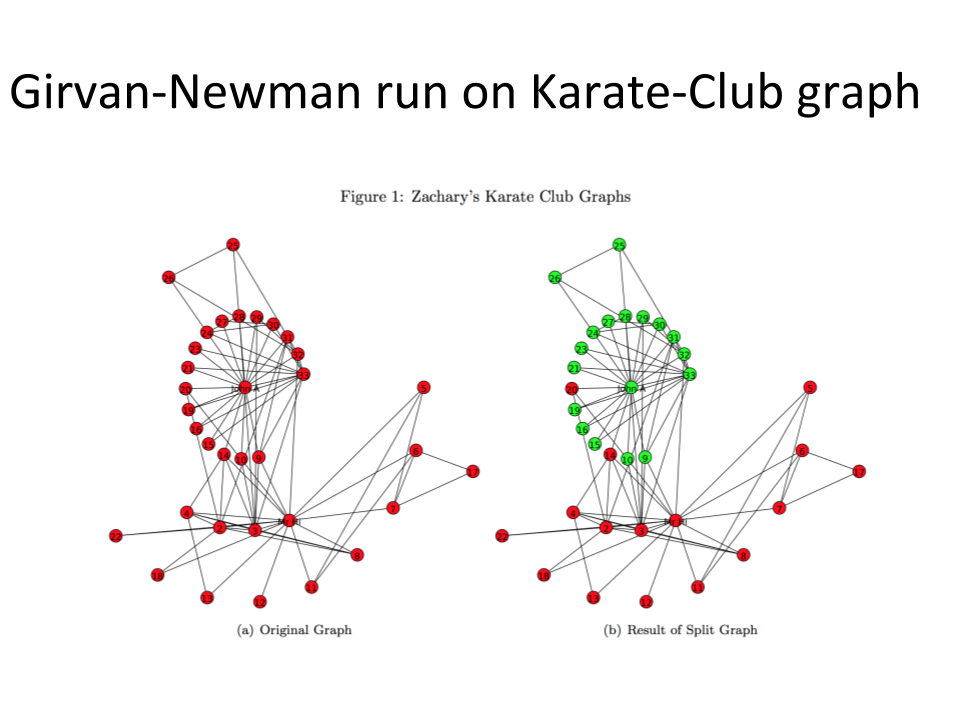
\includegraphics[width=\linewidth]{slide98.png} 
     \caption{Slide information from class}
  \end{subfigure}
  \caption{The karate club from 1977 class information.}
  \label{fig:comp1}
\end{figure}

Now let us compare what edges were removed using the Girvan-Newman algorithm and the edge betweenness algorithm I used with pyton coding.\\
\\
Table 1. Iterations compare edge removals\\
\begin{center}
  \begin{tabular}{ | c | c | c }
    \hline
     Iteration Number & Orignal Edge Removed & Edge Betweenness Removed\\ \hline
     1 & 0 32 & 0 31\\ \hline
     2 & 3 1 & 0 2 \\ \hline
     3 & 9 1 & 0 8 \\ \hline
     4 & 0 14 & 13 33 \\ \hline
     5 & 0 20 & 19 33 \\ \hline
     6 & 33 3 & 2 32\\ \hline
     7 & 2 31 & 1 30\\ \hline
     8 & 2 3 & 1 2\\ \hline
     9 & 3 4 & 2 3\\ \hline
     10 & 3 8 & 2 13\\ \hline
     11 & 3 14 & 2 7\\ \hline
     12 &  & 9 33\\ \hline
    \hline
  \end{tabular}
\end{center}
 
Since there is a chance that I may of used different numbers to represent people then what was used in the class slides.  I decide to count the number of nodes between the two split apart groups. I also decide to compare the pictures of both split apart groups.  Figure \ref{fig:comp2} shows the split of both my python edge betweenness and the class slide information.\\
\\
In the Edge Betweenness split one group had 15 the other had 19.
In the Class slide one group had 15 and the other had 19.  
So if the numbering is off comparing the date the number split of the nodes is correct.\\
\\
\begin{figure}[H]
  \centering
  \begin{subfigure}[b]{0.4\linewidth}
     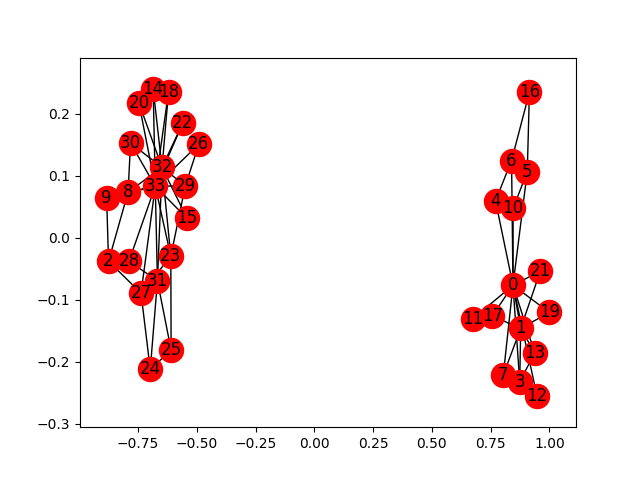
\includegraphics[width=\linewidth]{karate12.png}
     \caption{Edge Betweenness split apart}
  \end{subfigure}
  \begin{subfigure}[b]{0.4\linewidth}
     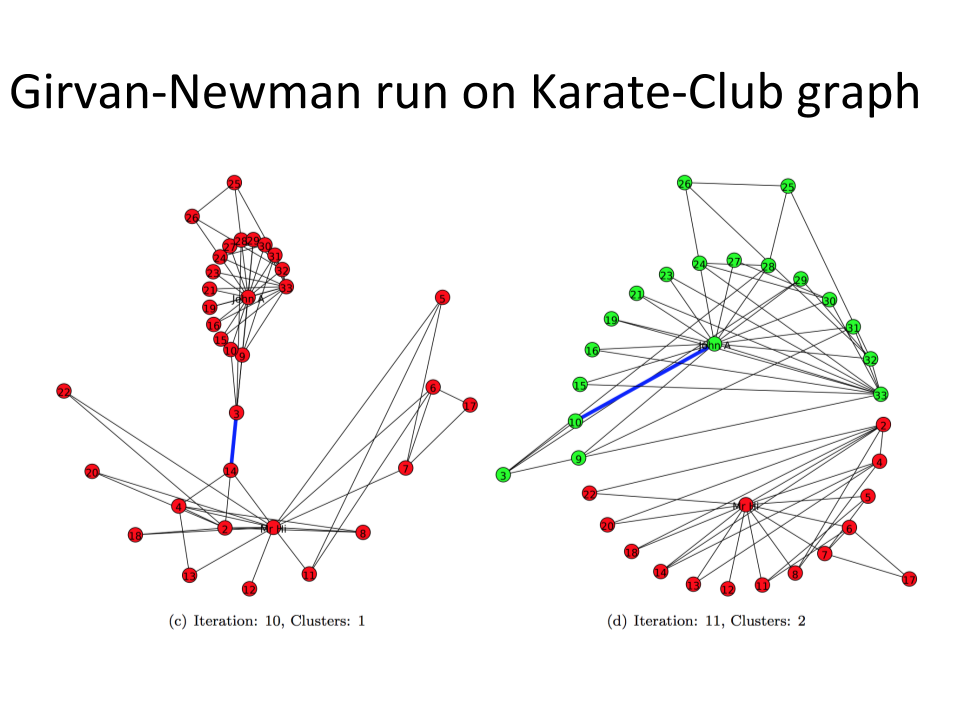
\includegraphics[width=\linewidth]{slide104.png} 
     \caption{Class slide information}
  \end{subfigure}
  \caption{The karate club from 1977 class information.}
  \label{fig:comp2}
\end{figure}


\pagebreak 
%----------------------------------------------------------------------------------------
%	Problem 2
%----------------------------------------------------------------------------------------
\section{Problem 2}
\subsection{Question 2}
(extra credit, 10 points)\\
\\
2. Use D3.js's force-directed graph layout to draw the Karate Club Graph before split. Color the nodes according to the factions they belong to (John A or Mr. Hi). After a button is clicked, split the graph based on the original graph split. Include a link to the HTML/JavaScript files in your report and all necessary screenshots.\\
\\
See: https://bl.ocks.org/mbostock/4062045\\
\\
https://d3js.org/\\
\\
\subsection{Answer 2}

\pagebreak
%----------------------------------------------------------------------------------------
%	Problem 3
%----------------------------------------------------------------------------------------
\section{Problem 3}
\subsection{Question 3}
(extra credit, 3 points)\\
\\
3.  We know the group split in two different groups.  Suppose the
disagreements in the group were more nuanced -- what would the clubs
look like if they split into groups of 3, 4, and 5?\\
\\
\subsection{Answer 3}

The class if using the Edge Betweenness split
If the class was to split into 3 groups using the Edge Betweenness split the figure \ref{fig:kart4}.  This took 15 iterations to great this group.\\
\\
\begin{figure}[h!]
  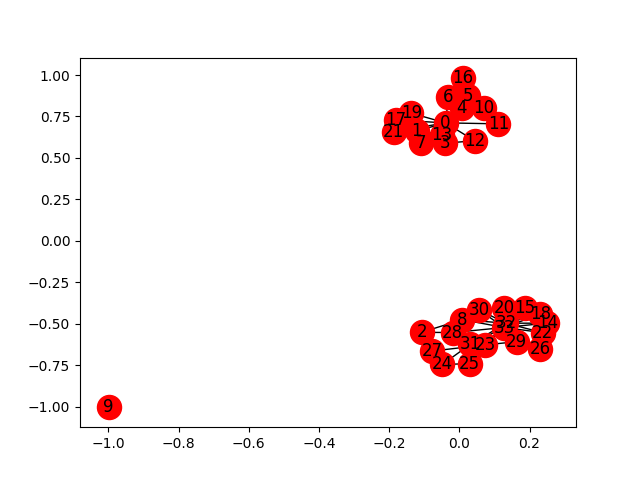
\includegraphics[width=\linewidth]{karate15.png}
  \caption{ Karate club in 3 groups}
  \label{fig:kart4}
\end{figure}

The class if using the Edge Betweenness split
If the class was to split into 4 groups using the Edge Betweenness split the figure \ref{fig:kart5}.  This took 19 iterations to great this group.\\
\\
\begin{figure}[h!]
  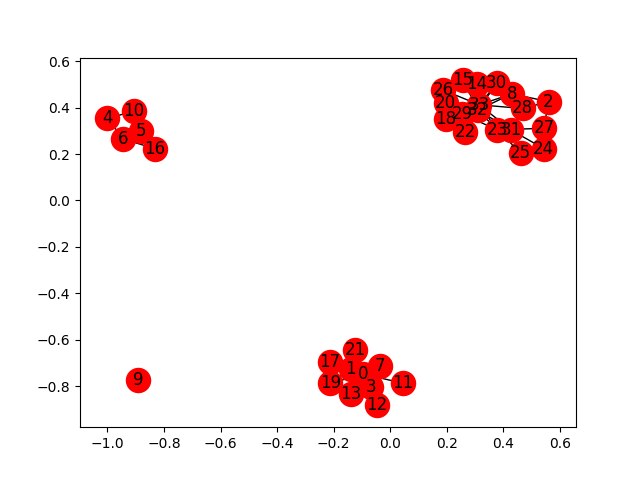
\includegraphics[width=\linewidth]{karate19.png}
  \caption{ Karate club into 4 groups}
  \label{fig:kart5}
 \end{figure}
  
The class if using the Edge Betweenness split
If the class was to split into 5 groups using the Edge Betweenness split the figure \ref{fig:kart6}.  This took 25 iterations to great this group.\\
\\
\begin{figure}[h!]
  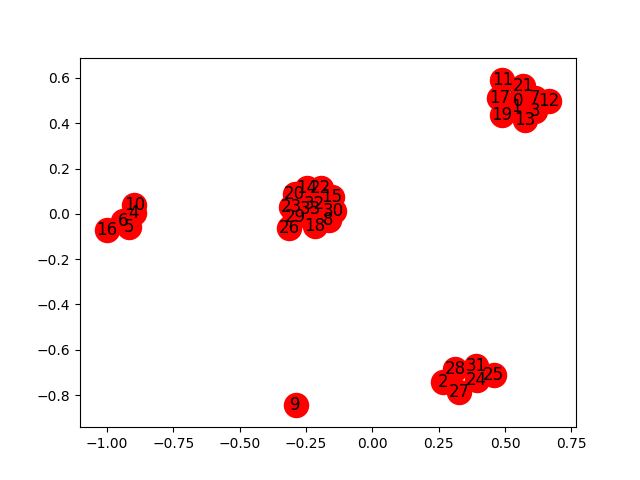
\includegraphics[width=\linewidth]{karate25.png}
  \caption{ Karate club into 5 groups}
  \label{fig:kart6}  
\end{figure}
\pagebreak

\end{document}
